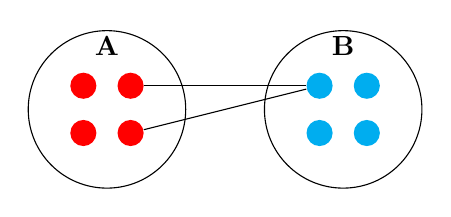
\begin{tikzpicture}
	\draw (-1.5,0) circle (1cm);
	\draw (-1.5,0.8) node {\textbf{A}};
	\draw ( 1.5,0) circle (1cm);
	\draw ( 1.5,0.8) node {\textbf{B}};
	
	\draw ( 1.2,  0.3) node[fill, cyan, circle] (a1) {};
	\draw ( 1.8, -0.3) node[fill, cyan, circle] (a2) {};
	\draw ( 1.8,  0.3) node[fill, cyan, circle] (a3) {};
	\draw ( 1.2, -0.3) node[fill, cyan, circle] (a4) {};
	
	\draw (-1.2,  0.3) node[fill, red, circle] (b1) {};
	\draw (-1.2, -0.3) node[fill, red, circle] (b2) {};
	\draw (-1.8,  0.3) node[fill, red, circle] (b3) {};
	\draw (-1.8, -0.3) node[fill, red, circle] (b4) {};
	
	\draw (a1) -- (b1);
	\draw (a1) -- (b2);
\end{tikzpicture}